\chapter{CMS Experiment}
\label{ch2}

\section{CMS detector}

The Compact Muon Solenoid (CMS) detector is one of the four interactions points on the LHC. It consist on different detectors made for different purposes, the silicon tracker, the electromagnetic calorimeter (ECAL), the hadron calorimeter (HCAL) the superconducting solenoid and the muon chamber. 
\\
\begin{figure}[h]
    \centering
     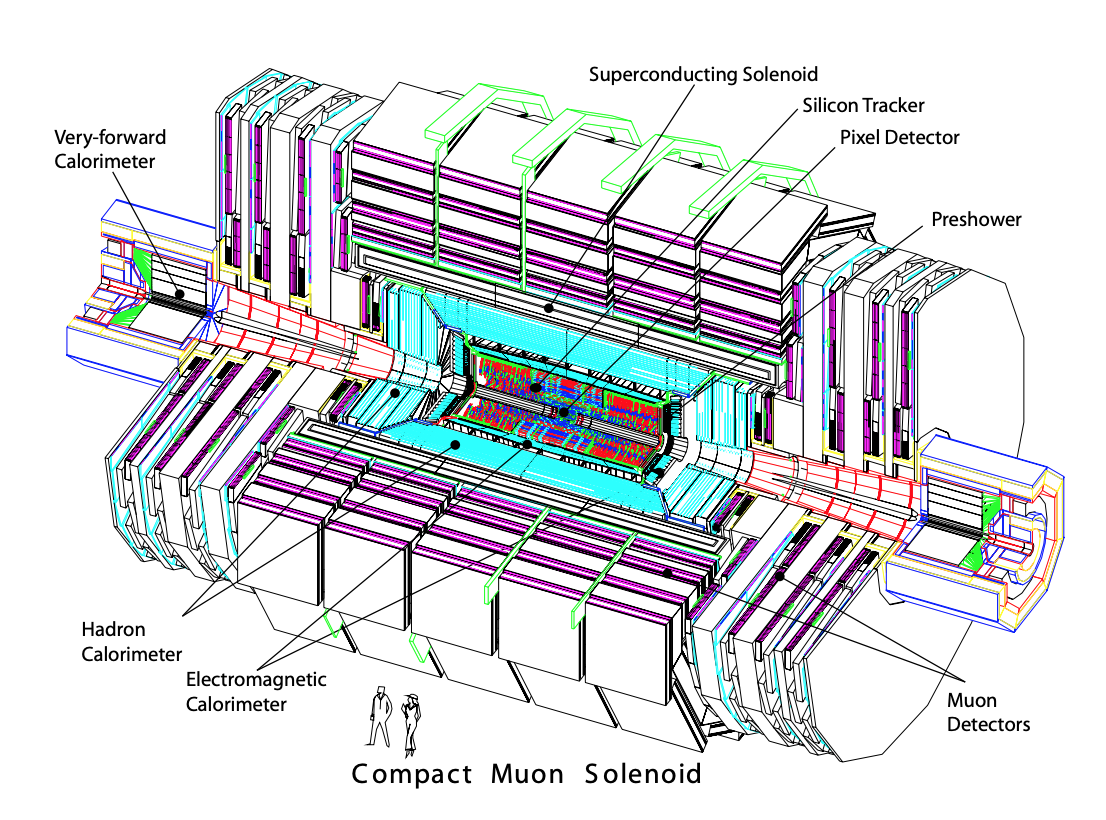
\includegraphics[width=1\textwidth]{cms2.png}
     \caption{The CMS detector size comparison with each of their components}
    \label{fig:four-forces}
\end{figure}

\\
The CMS has the form of a cylindrical onion with several concentric layers of components, this components are important to determine the properties of different particles all of this by bending their trajectories with a magnet that bend charged particles, this helps to identify the charges of the particles since they bend in different directions and allows to measure the momentum of a particle sine high momentum particles bend less than the low momentum ones. The principal magnet of the CMS is called Super Conducting Solenoid this magnet generates a field of about 4 Teslas and is very large 6.3m cold bore, 12.5 meters of length and 200 t of mass. The high magnetic field is confined to the volume of the detectors using the "return yoke", this yoke have a magnetic field strength of 2 Teslas and acts as the main support as well as the muon filter Its made of a high amount of steel and It weights more than 11000 tonnes.     \cite{CMS3}

One of the principal objectives of the CMS is identify with very high precision the paths taken by the particles that were bend by the magnetic field they called this part the inner tracker which is composed of different substructures, closest to the interaction point we have the Silicon Pixel Detector, then after the silicon strip detectors which are divided into the inner barrel part and the outer barrel part, the outer barrel and the outer end caps. When a charged particle pass through this layers interacts electromagnetically with the sensors leaving a hit that can be used to identify the path that a particle took. \cite{CMS1}

%Might update about the composition of this parts later.

Having information of the energy is important to understand what is happening at the collision point for this purpose there are two calorimeters on the CMS. The ECAL is made of 61200 lead tungstate crystals in the central barrel cap closed by 7324 crystals in the two of the endcaps in front of this crystals there is a press shower detector, the high density crystals allow  the calorimeter to be fast, have a fine granularity and being radiation resistant, Its capabilities are improved by the good crystal resolution which are provided by a homogeneous crystal calorimeter. It's surrounding the tracker and aims to measure the the energy of electrons, positrons or photons and stop them completely. The other calorimeter is the HCAL which is surrounding the ECAL and plays an essential role on the measurements of the energy of hadrons like the quarks, gluons, neutrinos and some exotic particles. which are also stopped here.  
\\

\begin{figure}[h]
    \centering
    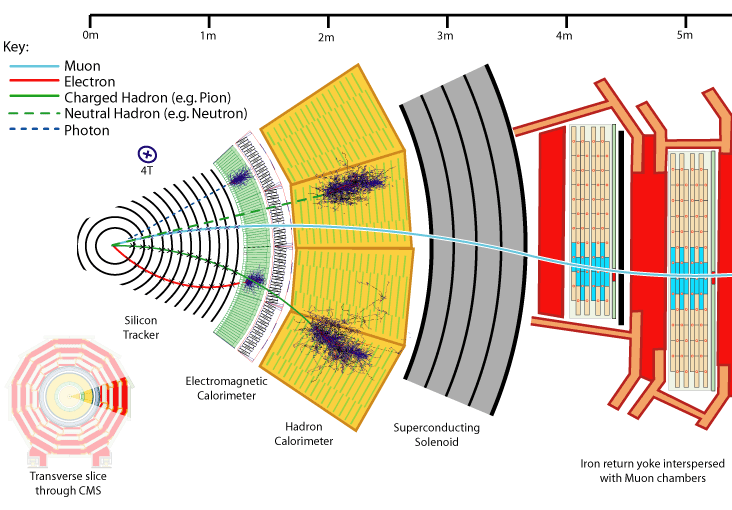
\includegraphics[width=1\textwidth]{cms.png}
     \caption{Different particles travelling across the different detectors of the CMS experiment}
    \label{fig:four-forces}
\end{figure}

\\
The CMS was optimized for the detections of muons and is the last particle that the CMS observe directly with the help of the muon chambers that is composed by many subdetectors which are interleaved with the return of the yoke of the solenoid located after the super conducting solenoid, muons are similar to electrons but 200 times heavier so they are not stopped by the calorimeters, the muon chambers have 3 main purposes; muon identification, momentum measurement and triggering. \cite{CMS2}

\section{Pixel Detector}

In the innermost part part of the CMS experiment there is a silicon pixel detector which is part of the tracking system. It has the task of provide high resolution 3D space points close to the collision point for track patter recognition and vertex reconstruction. It is located in a place where there is a harsh radiation environment giving Its high track density, in the CMS there was an pixel detector that was later changed during the first long shut down of the LHC during LS1 (2013-2014) and replaced by the CMS Phase-1 Pixel Detector in order to mantain efficient and robust tracking giving that with the upgrade of the accelerators the luminosity have doubled compared to the design value. It is expected that this detector to deliver high quality data until the end of the LHC Run 3 (Currently in process) after which the whole track detector on the CMS will be replaced.
   
Overall, is the closest detector to the beam pipe with cylindrical layers in the range of 3cm and 16cm at either end so It's vital to reconstruct the tracks of particles with very short live spans. It contains 124 millions pixels that allows to the tracking of the particles emerging from the collision with a extreme accuracy. It has 4 layers, each one of these layers is composed of silicon modules that are splitted into tiny silicon sensors this is what is called the pixels. These pixels have a size of 100 $\mu m$ -150 $\mu m$, when a charged particle pass through this pixels it gives the electrons on the silicon enough energy to be ejected with an applied voltage these charges are collected as a small signal which is amplified by an electronic readout ship. With these signals we can know which pixels were touched, allowing  us to recreate the track using the 2D tiles detectors and with the help of Its 4 layers can also generate a 3D picture. Nevertheless, the rate of the particles passing through this detectors is big at 3cm to the beam pipe the rate is about 600 million of particles $\cm^{2} / s$ the pixel detector is able to reconstruct all the tracks the particles leave behind. Each of the 124 million pixels are kept to a minimum power, even with only 50 microwatts per pixel the total power output of the whole detector is it about 7.5kW. It also has a freezing system of cooling tubes and kept about 20 degrees celsius reducing the damage to the modules made by the large stream of particles. 

The layout of the detector is optimized to have four hit coverage over the pseudorapidity range of  $|\eta| < 2.5$ which is important to improve the pattern recognition and track reconstruction and added redundancy to cope with hit loses. Apart from this the detector consist in the already mentioned four concentric barrel layers (L1-L4) with specific radius of 29mm, 68mm, 109 mm and 160 mm and three disks (D1-D3) on the ends with distances to the center of 291mm, 396mm and 516mm and the total silicon area is of 1.9 $m^{2}$. The detector is built from 1856 silicon sensor modules, 1184 of these are on the barrel pixel detectors (BPIX) and the rest one are on the forward pixel detectors (FPIX), each module consist in a sensor of 160x416 pixels connected to 16 readout chips (ROCs) for a total of 124 millions readout channels. \cite{pxd}

The BPIX and FPIX detectors are independent components, the BPIX consist in two half barrels with a length of 540mm each of the four layers are called half shells and is divided into two mechanically independent halves both composed of one half detector and two service half-cylinders. The FPIX is assembled from twelve disks which are divided into inner and outer half rings which supports 22 and 34 modules respectively and is divided into four mechanically independent quadrants each formed by three half-disks installed in a service half cylinder. This detectors are supplied with four service half-cylinders that hold the readout and control circuits.
\\
\begin{figure}[h]
    \centering
    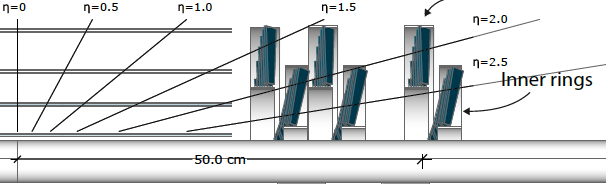
\includegraphics[width=1\textwidth]{pixeldetector.png}     
    \caption{Pixel detector outter rings and inner rings structure}
    \label{fig:PixelDetector}
\end{figure}

\\
In order to optimize the resolution of the tracking and the vertexing the materials used in the detector were minimized. Even with the additional layers the material budget for the CMS Phase-1 Pixel in the central region is almost the same as the original detector while reducing the forward region. This is possible thanks to the advanced nano carbon-fiber materials for the mechanical structure that adopt the usage of lower mass, and two phases $CO_{2}$ cooling systems. The electronics boards on the service half-cylinders are placed in higher pseudorapidity regions outside of the tracking acceptance. 

The innermost layer have to support high levels of radiation and hit rates a hadron fluence of $3.6x10^{15} n_{eq}/cm^{2}$ (neq is the units of 1 MeV of neutrons equivalent) is expected in the innermost layer after collecting a integrated luminosity of 500 $fb^{-1}$. In the outer layers of the BPIX and on the FPIX the expected hit rates are of about $600 MHz/cm^{2}$ for BPIX L1. 

The silicon detector modules is built from a planar silicon sensor bonded to an array of 2x8 ROCs. Each ROC is segmented on 4160 readout channels and reads information about each pixel. Since 2 ROCs can only be placed at a minimum distance between each other pixels along the ROC boundaries have twice the area and those at the corners have four times the area of a pixel, in the other side of the silicon sensor there is a high density interconnect (HDI). To simplify the module production as well Its maintenance, the same rectangular module geometry is used for both BPIX and FPIX detectors. In the BPIX detector the orientation of the sensor surface is parallel to the magnetic field, this means that the pixels are oriented parallel to the beam line. The FPIX detectors in the outer rings are rotated 20 degrees, in the inner ring the modules are arranged in an inverted cone array with an angle of 12 degrees respect to the beam line combined with the 20 degrees rotation. The orientation for the FPIX is made such as the long side of the pixels is in the radial direction.  

\\
\begin{figure}[h]
    \centering
    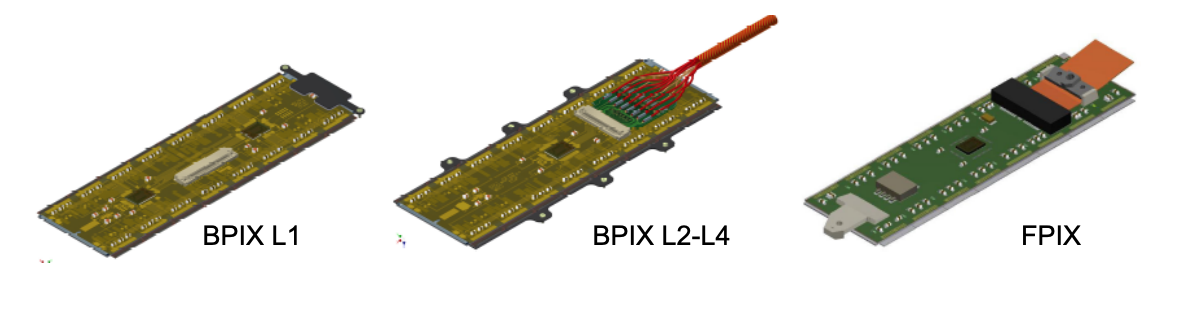
\includegraphics[width=1\textwidth]{BPIXFPIX.png}
    \caption{Barrel Pixel Detector moudles and Forward Pixel Detector Modules}
    \label{fig:BPIXFPIX}
\end{figure}

\\
The sensors of BPIX and FPIX were designed by two different companies, BPIX was made by CiS Forschungsinstitut fur Mikrosensorik in efurt on germany and FPIX was made on SINTEF micro-systems and sensors in Norway. The BPIX sensors were made on approximately 285 $\mu m$ of phosphorous-dope 4-inch wafers from silicon mono-crystals, all of this sensors were produced using silicon from the same ingot. In the other side, the FPIX sensors were made on 300 $\mu m$ thick 6 inch float-zone wafers, eight sensors were placed on one wafer, the wafers were accepted if at least six of It's sensors fulfill their specifications. 

The readout chips are made using 250 nm CMOS technology, this are named PSI46dig and PROC600. The PSI46dig is used on the outer BPIX layers (L2-L4) and in the FPIX detectors, meanwhile the PROC600 was designed for the innermost layer, taking into the consideration the expected hight hit rates. The single pixel efficiency of the PSI46dig at high rates was measured using internal calibration signal while exposing the ROCS to high-rate X-rays, the data loses for both of the detectors were of less thant 2 \% at the expected maximum hit rate of 120 MHz/$cm^{2}$ and the PROC600 efficiency is above 95 \% at rates up to 600 Mhz MHz/$cm^{2}$.

\section{Pixel Cluster Counting}

The Pixel Cluster Counting (PCC) method consist in counting the average number of pixel clusters on the detector to measure luminosity. This occurs during a zero bias event, an event that is trigged by requiring only that two proton bunches cross at the CMS interaction point. Giving that the number of pixels in really big the probability that a pixel is being hit by two different tracks by the same bunch crossing is really small. The mean number of pixel clusters in a simulated zero bias event is in the order of 100 per pp collision. The number of pixel clusters per bunch crossing is linearly dependent on pileup and therefore an accurate measure of the instantaneous luminosity.\cite{PCC1} The mean number of pixel cluster per trigger is \\ 


\begin{equation}
<N_{cluster}> = <N_{Pixel/Interaction}> <N_{interaction}> = <N_{Pixel/interaction}> \mu 
\end{equation}

here the $\mu$ is the number of interactions and with this the following equation and gives us a relation with the cross section $\simga_{i}$, instant luminosity and $\mu$

\begin{equation}
\mu = \frac{\sigma_{i}}{f}\frac{dL}{dt}
\end{equation}

here f is the frequency of the LHC, defining a new quantity $\simga_{cluster}$ = $\simga_{i}<N_{Pixel/Interaction}> $ and combining equation (2.1) and (2.2) we got

\begin{equation}
<N_{cluster}> = \frac{\sigma_{cluster}}{f} \frac{dL}{dt}
\end{equation}

Here, the value of $N_{cluster}$ is the mean number of pixel clusters on the pixel detector during a zero bias trigger at a head on period, the value of $\sigma_{cluster}$ can be obtained using the Van Der Meer scan and from the equation (2.3) we can obtain the luminosity from \cite{PCC2}

\begin{equation}
\sigma_{cluster} = <N_{cluster}> f (\frac{dL}{dt})^{-1}
\end{equation} 


\section{Pixel Detector Module Selection}

To be applicable to a van der mer scan the cluster cross section must use exactly the same detector configuration during the whole of the data taking and the calibration scan. This means if any of the modules of the detector didn't work at any point of the scans and didn't gave any readout It must be excluded from the calibration and the luminosity analysis, the stability of each module is determined in a ratio of module PCC and total PCC. \cite{PCC3}

From the total of 1856 modules on the pixel detector (1184 on the BPIX and 672 on FPIX) so in the analysis for the pcc vdm calibration onf 2024 for the fill 9639a total of 240 modules were used.


